\documentclass{article}
\usepackage{amsmath}
\usepackage{amssymb}
\usepackage{graphicx}
\usepackage{hyperref}
\usepackage[version=4]{mhchem}

\title{Problem 14}
\date{}

\begin{document}
\maketitle

\section*{Problem}
(2002 AMC 10A Problem 23) Points \(A, B, C\), and \(D\) lie on a line, in that order, with \(A B=C D\) and \(B C=12\). Point \(E\) is not on the line, and \(B E=C E=10\). The perimeter of \(\triangle A E D\) is twice the perimeter of \(\triangle B E C\). Find \(A B\).\\
(A) \(\frac{15}{2}\)\\
(B) 8\\
(C) \(\frac{17}{2}\)\\
(D) 9\\
(E) \(\frac{19}{2}\)\\
\centering
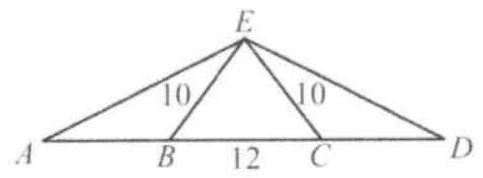
\includegraphics[width=\textwidth]{images/090(3).jpg}

\section*{Solution}
Solution not available.

\end{document}
